\chapter{Independently Controllable Factors}
\label{chapter:icf}
\section*{Article details}
Thomas V*, Bengio E*, Fedus W*, Pondard J, Beaudoin P, Larochelle H, Pineau J, Precup D, Bengio Y. ``Disentangling the independently controllable factors of variation by interacting with the world''. Presented at the \emph{ NeurIPS 2017 workshop on Learning Disentangled Representations: from Perception to Control} as an oral talk. 

Previous iterations of this paper have been presented at \emph{Reinforcement Learning and Decision Making (RLDM) 2017} and at the \emph{Montreal AI Symposium}.

\section*{Foreword}
This project began at first in January 2017 and led to several short papers and involved many authors from different institutions. The first one, ~\citet{bengio2017independently} was published at RLDM 2017, a subsequent and longer paper,~\citet{thomas2017independently} was presented at the Montreal AI Symposium 2017, and finally, a latter and more theoretically sound version, \citet{thomas2018disentangling} was presented as a spotlight paper in the NeurIPS 2017 workshop on Learning Disentangled Features: from Perception to Control.

The original motivation for this project is the way young children spontaneously learn to discover what they can do, how they can affect the world and the surrounding objects in a totally unsupervised manner~\citep{berlyne1966curiosity, gopnik1999scientist}. To do so, they associate aspects of the world they can control to a representation of such aspect -or object- in their brain. In this line of work, we looked at, in particular, aspects of the world that can be modified and represented indepedently from each other: we call them \textbf{independently controllable factors of variations}. This combines two objectives into one: (1) the agent has to discover without supervision a diverse set of policies it can execute, and (2) each policy must be mapped to a representation in the latent space.

The first point has been the focus of several works where, as in our work, the objective is similar to a mutual information criterion between the observed states and the label of the policy (or option/skill/context used)~\citep{still2012information, mohamed2015variational, gregor2016variational, florensa2017stochastic, eysenbach2018diversity, achiam2018variational}.

The second point, learning disentangled representation for reinforcement learning has been investigated by~\citet{anand2019unsupervised} where they annotate by hand \emph{attributes} of the world and learn a representation that shares a high mutual information with those attributes. In a more complex 3D world. \citet{eslami2018neural} learn a representation of a scene by encoding the information about different viewpoints at once. Works combining both the idea of exploring and learning a good representation of the world are more rare. We can cite \citet{kim2019emi}, where they use a mutual information objective to help exploration and learning of representation (this is however not unsupervised) and ~\citet{li2018disentangled} a follow-up work on the contribution presented here where they propose a simple mechanism to discover factors that cannot be controlled by the agent.

A very challenging aspect of this work was to be able to learn a diversity of meaningful factors. In the end, we always observed what we called a \emph{factor collapse} where a few interesting factors would be learned but many would remain undiscovered no matter the amount of training. While we were able to characterize and understand this problem very well, we did not manage at the time to solve it. Recently~\citet{strouse2021learning} proposed a solution to this issue by discriminating between \emph{aleatoric} and \emph{epistemic} uncertainties using an ensemble of neural networks, thus encouraging the system to be more curious about learning new factors rather than exploiting the ones already discovered.

\section*{Personal contribution}
\begin{itemize}
    \item Theoretical understanding of what objective ICF is optimizing. Making the link with (causal) mutual information
    \item Understanding and showcasing how our structured representation can be used for planning and inference
    \item Empirical validation (code + visualization) for most experiments presented in this paper.
\end{itemize}

\newpage

\begin{abstract}
    It has been postulated that a good representation is one that disentangles the underlying explanatory factors of variation. However, it remains an open question what kind of training framework could potentially achieve that. Whereas most previous work focuses on the static setting (e.g., with images), we postulate that some of the causal factors could be discovered if the learner is allowed to interact with its environment. The agent can experiment with different actions and observe their effects. More specifically, we hypothesize that some of these factors correspond to aspects of the environment which are independently controllable, i.e., that there exists a policy and a learnable feature for each such aspect of the environment, such that this policy can yield changes in that feature with minimal changes to other features that explain the statistical variations in the observed data. We propose a specific objective function to find such factors, and verify experimentally that it can indeed disentangle independently controllable aspects of the environment without any extrinsic reward signal.

\end{abstract}


\section{Introduction}

When solving Reinforcement Learning problems, what separates great results from random policies is often having the right feature representation. Even with function approximation, learning the right features can lead to faster convergence than blindly attempting to solve given problems \citep{jaderberg2016reinforcement}.

The idea that learning good representations is vital for solving most kinds of real-world problems is not new, both in the supervised learning literature \citep{Bengio-2009-book,Goodfellow-et-al-2016}, and in the RL literature \citep{dayan1993improving,precup2000temporal}. An alternate idea is that these representations do not need to be learned explicitly, and that learning can be guided through internal mechanisms of reward, usually called intrinsic motivation \citep{barto2004intrinsically,oudeyer2009intrinsic,salge2013empowerment, varintcontrol}. 

We build on a previously studied \citep{thomas2017independently} mechanism for representation learning that has close ties to intrinsic motivation mechanisms and causality. This mechanism explicitly links the agent's control over its environment to the representation of the environment that is learned by the agent. More specifically, this mechanism's hypothesis is that most of the underlying factors of variation in the environment can be controlled by the agent independently of one another. %

We propose a general and easily computable objective for this mechanism, that can be used in any RL algorithm that uses function approximation to learn a latent space. We show that our mechanism can push a model to learn to disentangle its input in a meaningful way, and learn to represent factors which take multiple actions to change and show that these representations make it possible to perform model-based predictions in the learned latent space, rather than in a low-level input space (e.g. pixels).

\section{Learning disentangled representations}

The canonical deep learning framework to learn representations is the autoencoder framework \citep{hinton2006reducing}. There, an encoder $f:S\to H$ and a decoder $g:H \to S$ are trained to minimize the \emph{reconstruction error}, $\|s-g(f(s))\|_2^2$. $H$ is called the latent (or representation) space, and is usually constrained in order to push the autoencoder towards more desirable solutions. For example, imposing that $H\in\mathbb{R}^K, S\in\mathbb{R}^N,\; K\ll N$ pushes $f$ to learn to compress the input; there the bottleneck often forces $f$ to extract the principal factors of variation from $S$. However, this does not necessarily imply that the learned latent space disentangles the different factors of variations. Such a problem motivates the approach presented in this work.




Other authors have proposed mechanisms to disentangle underlying factors of variation. Many deep generative models, including variational autoencoders~\citep{Kingma+Welling-ICLR2014} \remove{and other descendants of the Helmholtz machine~\citep{Dayan-et-al-1995}}, generative adversarial
networks~\citep{Goodfellow-et-al-NIPS2014} or non-linear versions of ICA~\citep{Dinh-et-al-2014,Hyvarinen+Morioka-NIPS2016} attempt to disentangle the underlying factors of variation by assuming that their joint distribution (marginalizing out the observed $s$) factorizes, i.e., that they are marginally independent.

Here we explore another direction, trying to exploit the ability of a learning agent to act in the world in order to impose a further constraint on the representation. We hypothesize that interactions can be the key to learning how to disentangle the various causal factors of the stream of observations that an agent is faced with, and that such learning can be done in an unsupervised way. %







\section{The selectivity objective}
We consider the classical reinforcement learning setting but in the case where extrinsic rewards are not available. We introduce the notion of \textbf{controllable factors of variation} $\phi \in \mathbb{R}^K$ which are generated from a neural network $\Phi(h, z), z \sim \mathcal{N}(0, 1)^m$ where $h = f(s)$ is the current latent state. The factor $\phi$ represents an embedding of a policy $\pi_\phi$ whose goal is to realize the variation $\phi$ in the environment.

To discover meaningful factors of variation $\phi$ and their associated policies $\pi_\phi$, we consider the following general quantity $\mathcal{S}$ which we refer to as selectivity and that is used as a reward signal for $\pi_\phi$:
\begin{equation}
    \mathcal{S}(h, \phi) = \mathbb{E}  \left[\log \frac{A(h', h, \phi)}{\mathbb{E}_{p(\varphi|h)}[A(h', h, \varphi)]} \;\big|\; \; {s' \sim \rmP^{\pi_\phi}_{ss'}}\right]
      \label{eq:general-selectivity}
\end{equation}

Here $h=f(s)$ is the encoded initial state before executing $\pi_\phi$ and   $h' = f(s')$ is the encoded terminal state. $\phi$ and $\varphi$ represent factors of variation a \emph{factor}.
$A(h', h, \phi)$ should be understood as a score describing how close $\phi$ is to the variation it caused in $(h', h)$. For example in the experiments of section 4.1, we choose $A$ to be a gaussian kernel between $h'-h$ and $\phi$, while in the experiments of section 4.2, we choose $A(h', h, \phi) = \max\{0,\langle h'-h, \phi \rangle\}$.
The intuition behind these objectives is that in expectation, a factor $\phi$ should be close to the variation it caused $(h', h)$ when following $\pi_\phi$ compared to other factors $\varphi$ that could have been sampled and followed thus encouraging \textbf{independence} within the factors.


Conditioned on a scene representation $h$, a distribution of policies are feasible. Samples from this distribution represent ways to modify the scene and thus may trigger an internal selectivity reward signal. For instance, $h$ might represent a room with objects such as a light switch. $\phi = \phi(h,z)$ can be thought of as the distributed representation for the ``name'' of an underlying factor, to which is associated a policy and a value.  In this setting, the light in a room could be a factor that could be either on or off. It could be associated with a policy to turn it on, and a binary value referring to its state, called an attribute or a feature value.%
We wish to jointly learn the policy $\pi_\phi(\cdot|s)$ that modifies the scene, so as to control the corresponding value of the attribute in the scene, whose variation is computed by a scoring function $A(h', h, \phi) \in \mathbb{R}$. In order to get a distribution of such embeddings, we compute $\phi(h,z)$ as a function of $h$ and some random noise $z$.




The goal of a selectivity-maximizing model is to find the density of factors $p(\phi |h)$, the latent representation $h$, as well as the policies $\pi_\phi$ that maximize $\mathbb{E}_{p(\phi|h)} [\mathcal{S}(h, \phi)]$.



\begin{figure}
\centering
{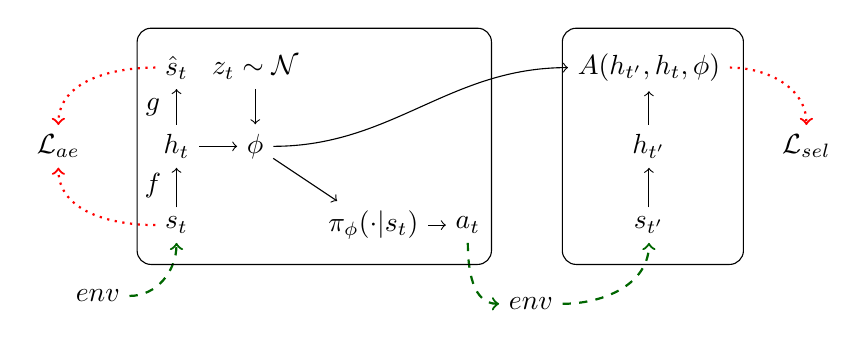
\begin{tikzpicture}

\def \pA {0}
\def \pB {6}
\def \pmid {2.5}

\node[] (st) at (\pA,0) {$s_t$};
\node[] (ht) at (\pA,1) {$h_t$};
\node (st_rec) at (\pA,2) {$\hat{s}_t$};

\draw[->,draw=black] (st) to (ht);
\draw[->,draw=black] (ht) to (st_rec);
\node at (-.3,1.5) {$g$};
\node at (-.3,0.5) {$f$};

\node (env) at (-1,-0.9) {$env$};
\draw[->,draw=black!60!green,dashed,thick] (env) to[out=0,in=-90] (st);


\node[] (st1) at (\pB,0) {$s_{t'}$};
\node[] (ht1) at (\pB,1) {$h_{t'}$};
\draw[->,draw=black] (st1) to (ht1);

\node[] (pi0) at (\pmid,0) {$\pi_\phi(\cdot|s_t)$};
\node[] (phi0) at (\pmid-1.5,1) {$\phi$};
\node[] (z0) at (\pmid-1.5,2) {$z_t \sim \mathcal{N}$};
\node[] (A1) at (\pB,2) {$A(h_{t'}, h_t,\phi)$};
\draw[->,draw=black] (z0) to (phi0);
\draw[->,draw=black] (ht) to (phi0);
\draw[->,draw=black] (phi0) to (pi0);
\draw[->,draw=black] (phi0) to[in=180,out=0] (A1);
\draw[->,draw=black] (ht1) to (A1);

\begin{scope}[]

\end{scope}
\node[] (aT) at (\pmid+1.2,-0) {$a_t$};
\node[] (env1) at (\pmid+2,-1) {$env$};
\draw[->] (pi0) to (aT);
\draw[->,draw=black!60!green,dashed,thick] (aT) to[out=-90,in=180] (env1);
\draw[->,draw=black!60!green,dashed,thick] (env1) to[out=0,in=-90] (st1);

\node[] (lossAE) at (\pA-1.5,1) {$\mathcal{L}_{ae}$};
\draw[->,draw=red,dotted,thick] (st) to[out=180,in=-90] (lossAE);
\draw[->,draw=red,dotted,thick] (st_rec) to[out=180,in=90] (lossAE);

\node[] (lossSel) at (\pB+2,1) {$\mathcal{L}_{sel}$};
\draw[->,draw=red,dotted,thick] (A1) to[out=0,in=90] (lossSel);

\draw
  {[rounded corners=5pt](-0.5,-0.5)  --
  (\pmid+1.5,-0.5)  -- 
  (\pmid+1.5,2.5) --
  (-0.5,2.5) --
  cycle};
\draw
  {[rounded corners=5pt](-1.1+\pB,-0.5)  --
  (1.2+\pB,-0.5)  -- 
  (1.2+\pB,2.5) --
  (-1.1+\pB,2.5) --
  cycle};
\end{tikzpicture}}
\caption{The computational model of our architecture. $s_t$ is the first state, from its encoding $h_t$ and a noise distribution $z$, $\phi$ is generated. $\phi$ is used to compute the policy $\pi_\phi$, which is used to act in the world. The sequence $h_t,h_{t'}$ is used to update our model through the selectivity loss, as well as an optional autoencoder loss on $h_t$.}
\end{figure}



\subsection{Link with mutual information and causality}
The selectivity objective, while intuitive, can also be related to information theoretical quantities defined in the latent space.
From \citep{donsker1975asymptotic,ruderman2012tighter} we have
$\kl{p}{q} = \sup_{A\in \mathcal{L}^\infty(q)} \mathbb{E}_p [ \log A] - \log \mathbb{E}_q [A]$.
Applying this equality to the mutual information $\mathcal{I}_p(\phi, h' | h) = \mathbb{E}_{p(h'|h)}\big[ \kl{p(\phi|h', h)}{p(\phi|h)}\big]$
gives
$$\mathcal{I}_p(\phi, h' | h) \ge \sup_\theta  \mathbb{E}_{p(\phi|h)} \big[ \mathcal{S}(h, \phi)\big]$$
where $\theta$ is the set of weights shared by the factor generator, the policy network and the encoder.

Thus, our total objective along entire trajectories is a lower bound on the causal \citep{ziebart2010modeling} or directed \citep{massey1990causality} information $\mathcal{I}_p(\phi \mapsto h) = \sum_t \mathcal{I}_p(\phi_{1:t}, h_t|h_{t-1})$ which is a measure of the \textbf{causality} the process $\phi$ exercises on the process $h$. See Appendix \ref{appendix:bound} for details.



\section{Experiments}
\remove{\color{red} So do we
\begin{enumerate}
\item Keep only this experiment (we wouldn't have to worry much about the space but that is light on the experiments)
\item Add the one with planning/policy inference?~\ref{sec:exp-mb-ppi} (small example from the paper)
\item Add the one with factors that seem to like to toggle switch in multistep~\ref{sec:multistep} (though not the behaviour we would really expect)
\item Add the discrete one?~\ref{sec:sel-only}
\end{enumerate}
Seems the experiments is working, doing a figure....}
We use MazeBase~\citep{sukhbaatar2015mazebase} to assess the performance of our approach. We do not aim to solve the game.
In this setting, the agent (a red circle) can move in a small environment ($64 \times 64$ pixels) and perform the actions \texttt{down, left, right, up}. The agent can go anywhere except on the orange blocks.




\subsection{Learned representations}

\begin{figure}
\centering
\begin{subfigure}{.45\textwidth}
{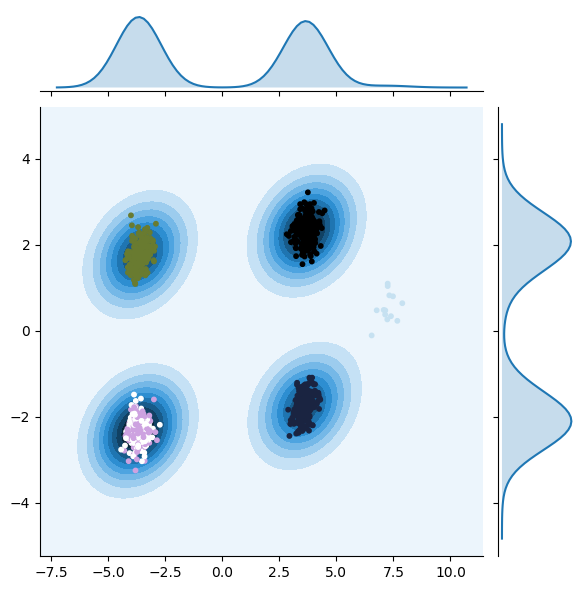
\includegraphics[width=0.9\linewidth]{articles/icf/figures/23000_kde_dh.png}}
\end{subfigure}
\centering
\begin{subfigure}{.45\textwidth}
{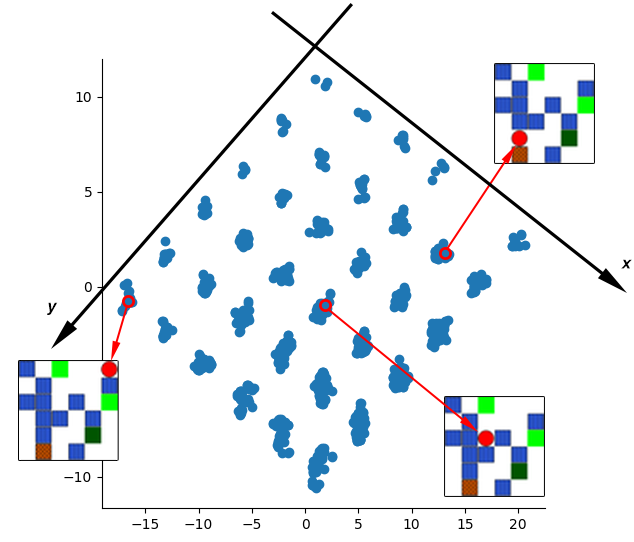
\includegraphics[width=0.9\linewidth]{articles/icf/figures/disentangle-kdeh.png}} %
\end{subfigure}

\caption{(a) Sampling of $1000$ variations $h' - h$ and its kernel density estimation encountered when sampling random controllable factors $\phi$. We observe that our algorithm disentangles these representations on $4$ main modes, each corresponding to the action that was actually taken by the agent.\protect\footnotemark
\, (b) The disentangled structure in the latent space. The $x$ and $y$ axis are disentangled such that we can recover the $x$ and $y$ position of the agent in any observation $s$ simply by looking at its latent encoding $h = f(s)$. The missing point on this grid is the only position the agent cannot reach as it lies on an orange block.}
\label{fig:dis_space}
\end{figure}

\footnotetext{pink and white for \texttt{up}, light blue for \texttt{down+left}, green for \texttt{right}, purple black \texttt{down} and night blue for \texttt{left}.}

After jointly training the reconstruction and selectivity losses, our algorithm disentangles four directed factors of variations as seen in Figure~\ref{fig:dis_space}: $\pm x$-position and $\pm y$-position of the agent. For visualization purposes we chose the bottleneck of the autoencoder to be of size $K = 2$.
To complicate the disentanglement task, we added the redundant action \texttt{up} as well as the action \texttt{down+left} in this experiment.

The disentanglement appears clearly as the latent features corresponding to the $x$ and $y$ position are orthogonal in the latent space. Moreover, we notice that our algorithm assigns both actions \texttt{up} (white and pink dots in Figure~\ref{fig:dis_space}.a) to the same feature. It also does not create a significant mode for the feature corresponding to the action \texttt{down+left} (light blue dots in Figure~\ref{fig:dis_space}.a) as this feature is already explained by features \texttt{down} and \texttt{left}.



\subsection{Towards planning and policy inference}
\label{sec:exp-mb-ppi}

This disentangled structure could be used to address many challenging issues in reinforcement learning. We give two examples in figure~\ref{fig:prediction_recovering}: 
\begin{itemize}
\item Model-based predictions: Given an initial state, $s_0$, and an action sequence $a_{\{0:T-1\}}$, %
we want to predict the resulting state $s_T$.

\item A simplified deterministic policy inference problem: Given an initial state $s_{start}$ and a terminal state $s_{goal}$, we aim to find a suitable action sequence $a_{\{0:T-1\}}$ such that $s_{goal}$ can be reached from $s_{start}$ by following it.
\end{itemize}
Because of the $tanh$ activation on the last layer of $\phi(h, z)$, the different factors of variation $dh = h' - h$ are placed on the vertices of a hypercube of dimension $K$, and we can think of the the policy inference problem as finding a path in that simpler space, where the starting point is $h_{start}$ and the goal is $h_{goal}$. We believe this could prove to be a much easier problem to solve.

\begin{figure}[t]
\centering
\begin{subfigure}{.45\textwidth}
\centering
{\scalebox{.6}{
\begin{tikzpicture}
\node[inner sep=0pt] (im0) at (0,0)
    {\fbox{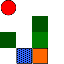
\includegraphics[width=.25\textwidth]{articles/icf/figures/im0_good.png}}};
\node[inner sep=0pt] (im1) at (5,0)
    {\fbox{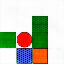
\includegraphics[width=.25\textwidth]{articles/icf/figures/im1_good.png}}};


\node[] (ht) at (0,-4) {$\underbrace{h}_{(0.4,\ 13.1)}$};
\node[] (ht1) at (7,-4) {$\underbrace{\hat{h'}}_{(-4.6,\ -1.9)} = h + \underbrace{dh_{{\color{right} {\color{right} right}}}}_{(5,\ -5)} + \underbrace{2\cdot dh_{{\color{down} down}}}_{(-10,\ -10)}$}; 
    \draw[->,thick] (im0.south) -- (ht.north)
    node[midway,fill=white] {Encoder};
    \draw[->,thick] (5, -3.3) -- (im1.south)
    node[midway,fill=white] {Decoder};
    
    \draw[->,thick] (ht.east) -- (ht1.west);
    
\end{tikzpicture}}}
\end{subfigure}
\begin{subfigure}{.45\textwidth}
\centering
{\scalebox{.6}{
\begin{tikzpicture}
\node[inner sep=0pt] (im0) at (0,0)
    {\fbox{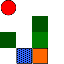
\includegraphics[width=.25\textwidth]{articles/icf/figures/im_causal0_good.png}}};
\node[inner sep=0pt] (im1) at (5,0)
    {\fbox{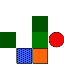
\includegraphics[width=.25\textwidth]{articles/icf/figures/im_causal1_good.png}}};


\node[] (ht) at (0,-3.5) {$\underbrace{h_1}_{(0.4,\ 13.1)}$};
\node[] (ht1) at (5,-3.5) {$\underbrace{h_2}_{(5.9,\ -11.6)}$}; 
\node[] (dh) at (2.5,-5) {$dh ={(5.5,\ -24.8)} \approx 2\cdot dh_{{\color{down} down}} + 3\cdot dh_{{\color{right} right}}$};
    \draw[->,thick] (im0.south) -- (ht.north)
    node[midway,fill=white] {Encoder};
    \draw[<-,thick] (ht1) -- (im1.south)
    node[midway,fill=white] {Encoder};
    
    \draw[->,thick] (ht.east) -- (dh.north);
     \draw[->,thick] (ht1.west) -- (dh.north);
    
\end{tikzpicture}}
} %
\end{subfigure}
\caption{(left) Predicting the effect of a cause on Mazebase. The leftmost image is the visual input of the environment, where the agent is the round circle, and the switch states are represented by shades of green. After the training, we are able to distinguish one cluster per $dh$ (Figure \ref{fig:dis_space}), that is to say per variation obtained after performing an action, independently from the position $h$. Therefore, we are able to move the agent just by adding the corresponding $dh$ to our latent representation $h$. The second image is just the reconstruction obtained by feeding the resulting $h'$ into the decoder. (right) Given a starting state and a goal state, we are able to decompose the difference of the two representations $dh$ into a (non-directed) sequence of movements.}
\label{fig:prediction_recovering}
\end{figure}


However, this disentangled representation alone cannot solve completely these two issues in an arbitrary environment. Indeed, the only factors we are able to disentangle are the factors directly \textit{controllable} by the agent, thus, we are not able to account for the ambient dynamics or other agents' influence.



\subsection{Multistep embedding of policies}
In this experiment, $\phi$ are embeddings of $3$-steps policies $\pi_\phi$. We add a model-based loss $\mathcal{L}_{MB}=||h_{t+3} - T_\theta(h_t, \phi)||^2$ defined only in the latent space, and jointly train a decoder alongside with the encoder. Notice that we never train our model-based cost at pixel level.
While we currently suffer from mode collapsing of some factors of variations, we show that we are successfully able to do predictions in latent space, reconstruct the latent prediction with the decoder, and that our factor space disentangles several types of variations.

\begin{figure}
\centering
\begin{subfigure}{.45\textwidth}
{{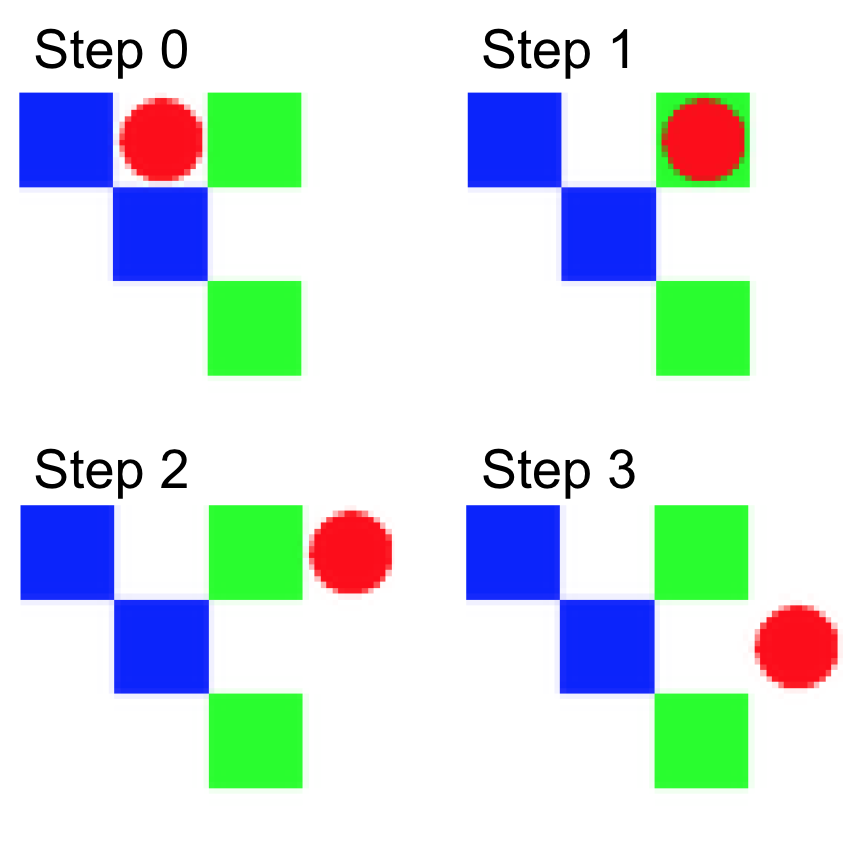
\includegraphics[width=.65\linewidth]{articles/icf/figures/square_traj.png}}} %
\end{subfigure}
\begin{subfigure}{.45\textwidth}
{{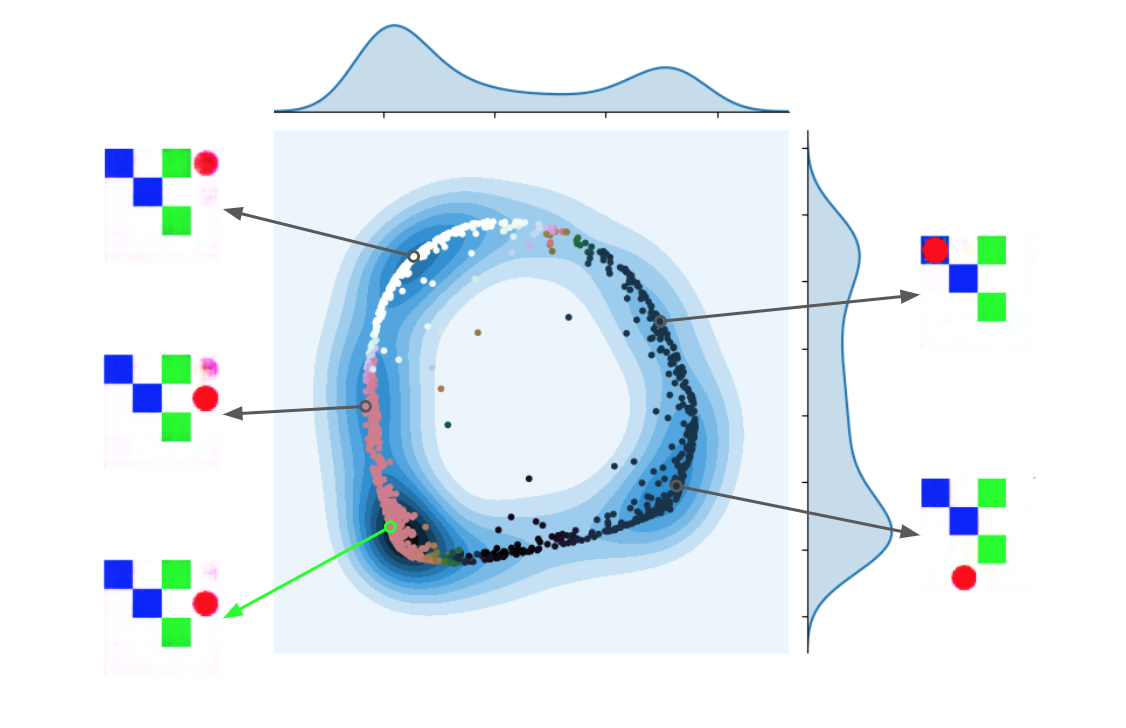
\includegraphics[width=.90\linewidth]{articles/icf/figures/phi_space.png}}}
\end{subfigure}

\caption{(a) The actual 3-step trajectory done by the agent. (b) PCA view of the space $\phi(h_0, z), z \sim \mathcal{N}(0,1)$. Each arrow points to the reconstruction of the prediction $T_\theta(h_0, \phi)$ made by different $\phi$. The $\phi$ at the start of the green arrow is the one used by the policy in (a). Notice how its prediction accurately predicts the actual final state.}
\end{figure}





\section{Conclusion, success and limitations}
Pushing representations to model independently controllable features currently yields some encouraging success. Visualizing our features clearly shows the different controllable aspects of simple environments, yet, our learning algorithm is unstable. What seems to be the strength of our approach could also be its weakness, as the independence prior forces a very strict separation of concerns in the learned representation, and should maybe be relaxed.

Some sources of instability also seem to slow our progress: learning a conditional distribution on controllable aspects that often collapses to fewer modes than desired, learning stochastic policies that often optimistically converge to a single action, tuning many hyperparameters due to the multiple parts of our model. Nonetheless, we are hopeful in the steps that we are now taking. Disentangling happens, but understanding our optimization process as well as our current objective function will be key to further progress. 